% ---- ETD Document Class and Useful Packages ---- %
\documentclass{ucetd}
\usepackage{subfigure,epsfig,amsfonts}
\usepackage{natbib}
\usepackage{amsmath}
\usepackage{amssymb}
\usepackage{amsthm}
\graphicspath{ {figures/ch1/} }
\begin{document}


\chapter{Introduction}
\section{Background}
%Brief intro to quantitative Biology
Biologists have long been fascinated by the myriad beautiful movements that give form and function to developing organisms \cite{Thompson:1917up}.  Starting from a single fertilized embryo, cell growth, cell division, cell migration, and various cell shape changes facilitate the formation of increasingly complex tissues and organs.  Using ideas from classical physics, early researchers during the so-called \textit{Entwicklungsmechanik} (developmental mechanics) period sought to explain how mechanical forces such as spring forces, osmotic pressure, shear stresses, and surface tension can drive various tissue movements during embryonic development.  During the early 1950's, the field of developmental biology took a large step forward when the great mathematician Alan Turing published his seminal paper on morphogenesis \cite{Turing:1952vn}.  Turing demonstrated that a simple system of reacting and diffusing chemical \textit{morphogens} could generate robust spatial patterns \cite{Turing:1952vn}.  It is likely that Turing would have extended his mathematical theory of chemical-based pattern formation to describe the morphogenetic movements of cells and tissues were it not for his untimely death \cite{Turing:1952vn, Howard:2011da}.  Indeed, we now know that the the forces that cells generate, and the resulting embryonic shape changes, are the result of a multitude of interacting components that are both chemically and mechanically regulated \cite{Mammoto:2010bt}.





%Biophysical Tools
Our understanding of embryonic development has greatly improved in the intervening years since the \textit{Entwicklungsmechanik} period.  Decades of research have uncovered many of the key genetic and biochemical pathways underlying the organization of the animal body plan.  Recent advances in light microscopy, the discovery of fluorescent proteins, and the creation of novel biophysical tools now gives researchers unprecedented access to interrogating the inner mechanical and biochemical workings of cells \cite{Heisenberg:2013jk}.  Coupled with high-resolution live imaging, fluorescent probes such as green fluorescent protein (GFP) can be used to assay the expression, activity, and localization patterns of force regulating molecules in cells and tissues.  Particle tracking techniques have been developed to measure the motion of individual proteins, as well as aggregates of molecules.  For example, single-molecule imaging can be used to measure the rates at which various GFP-tagged molecules associate with, and dissociate from, the cell surface \cite{Robin:2014jf}.  Single-molecule imaging can also be used to measure the local cell surface deformation rate during shape changes  (see Chapter 2).  The recent invention of optogenetic probes will also help researchers shed light on the spatial and temporal regulation of signalling pathways that control force generation \cite{Wagner:2016ev}.   Now, one of the major challenges facing cell and developmental biologists will be to use these new tools to understand how the formation of complex tissue architectures is driven by underlying genetic and biochemical mechanisms, as well as the concerted deformation, compression, elongation, and rearrangement of individual cells.




%Specific instances of cell shape changes
Individual cells have the ability to pattern their force-generating machinery in order to change their shape for accomplishing specific tasks \cite{Lecuit:2011ec}.  For example, during cell division an animal cell first rounds up, positions its furrow, and then constricts its membrane in order to split into two daughter cells \cite{Srivastava:2016dm}.  Neuronal cells polarize by extending long axons and several smaller dendrites, thus providing a means for signals to be transmitted throughout the nervous system  \cite{Stiess:2011ji}.  Cell migration, which is important for wound healing, chemotaxis, and immune responses, occurs when a recently polarized cell propels itself forward by forming protrusions to extend its leading edge and by contracting to retract its trailing edge \cite{Mayor:2016iw}.


%Morphogenetic movements that result from specific instances of cell shape changes
Individual cells can also coordinate their shape changes in order to bend, rearrange, elongate, and move epithelial tissues during morphogenesis \cite{Heisenberg:2013jk,Lecuit:2011ec}.  The forces that generate individual cell shape changes are integrated and transmitted throughout a developing tissue by adhesive interactions between neighboring cells, and between cells and external substrates.  For example, apical constriction of epithelial cells is a common morphogenetic movement that has been shown to drive epithelial sheet bending and invagination in diverse developmental contexts such as vertebrate neural tube formation and gastrulation in \textit{Drosophila melanogaster} and \textit{Caenorhabditis elegans} \cite{Sawyer:2010ku,Keller:2011dm}.  Spatiotemporal coordination of epithelial cell migration is one of the key requirements for proper cell intercalation, which is thought to drive tissue narrowing and elongation \cite{WalckShannon:2014go}.  

%Molecular basis for force generation
The various cell shape changes and movements described above all appear to be very different mechanisms that operate in distinct cellular and developmental contexts.  However, much experimental work has demonstrated that all of these cells use cortical actomyosin networks to generate the forces necessary to change their shape \cite{Lecuit:2007cw,Salbreux:2012bo}.  Cortical actomyosin networks sit just below the membrane of embryonic and epithelial cells, and are composed of non-muscle myosin II motors, actin filaments, and a host of bundling, cross-linking, capping, and severing proteins \cite{Levayer:2012bu,Murrell:2015kt}.  Like the sarcomeric structures found in muscle cells, cortical actomyosin networks generate force when non-muscle myosin II uses the energy from ATP hydrolysis to slide actin filaments of opposite polarity past each other.  However, unlike the relatively stable sarcomeres, the individual components of cortical actomyosin networks are constantly turning over and being redistributed whenever the network generates force.  This allows cells to rapidly reorganize their cortical actomyosin networks into structures such as cytokinetic rings, branched lamellar networks, and stress fibers.  Recent evidence suggests that force generation within cortical actomyosin networks might also regulate the distribution of biochemical regulators of contractility \cite{Munro:2004jk}.  Therefore, understanding how local force generation leads to cell shape changes will require a study of the interplay between biochemical signalling and cortical actomyosin contractility. 


%The purpose of this thesis
The subject of this thesis is an increasingly common form of cell shape change known as pulsatile shape change, or pulsed contractility \cite{Munro:2004jk,Martin:2009du,Gorfinkiel:2016bv}.  Pulsatile cell shape changes have been observed during various developmental events such as gastrulation in \textit{Drosophila} and \textit{C. elegans}, compaction of the early mouse embryo, and convergence extension in \textit{Xenopus} \cite{Martin:2009du, RohJohnson:2012cf,Maitre:2015hc}.  The purpose of the remainder of this chapter is to provide a biological context for the novel findings reported in this dissertation.  First, I will provide an overview of the structure and regulation of various components of the actomyosin cortex.  Second, I will provide a brief review of the recent pulsed contraction literature during early \textit{Drosophila} development.  Then, I will describe conceptual and mathematical models that others in the field have proposed to describe the initiation and termination of pulsed contractions.  Finally, I will give a preview of the approach that I (in collaboration with members of the Munro lab) have taken to uncovering important mechanisms regulating pulsed contractility.



\section{Assembly and regulation of actomyosin networks}

\subsection{Structure and regulation of Myosin II}

%Myosin overview
Myosins are a diverse superfamily of actin-based molecular motor proteins that regulate force generation and translocation in cells and tissues \cite{Sellers:2000ub,VicenteManzanares:2009ik}.  A comparative genomic analysis has revealed that there are at least 35 different myosin classes, 13 of which are found in humans \cite{Odronitz:2007hn,Sweeney:2010fg}.  Most myosins consist of an N-terminal head or motor domain, a neck domain, and a C-terminal tail domain \cite{Mooseker:2007ij}.  The head domain binds and hydrolyzes ATP in an actin-dependent manner.  The neck domain contains one or more IQ motifs which bind calmodulin family proteins, such as myosin light chains.  In some cases, different IQ motifs within a single myosin are able to simultaneously bind different light chains (e.g. class II myosins).  The tail domains function by binding cargo for intracellular transport and/or promoting the dimerization of the heavy chain \cite{Sellers:2000ub}.  Myosins within each class often share a similar tail structure \cite{Krendel:2005ko}.  At the molecular scale, myosin motors exhibit a wide range of dynamic behaviors that include sliding, pulling, and walking along actin filaments.  These molecular behaviors translate into the different myosins regulating many different processes such as muscle contraction, cell division, cell migration, adhesion, cell polarity, intracellular trafficking, and organelle positioning \cite{Sellers:2000ub,VicenteManzanares:2009ik}.  



%Power stroke, duty ratio, and 
All myosin motors use a conserved mechanism to convert chemical energy into mechanical energy by coupling ATP hydrolysis to cycles of actin attachment and detachment \cite{DeLaCruz:2004fq}.  In the presence of ADP (i.e., the absence of hydrolyzable ATP), the myosin motor domain binds tightly to an actin filament.  The subsequent exchange of ADP for ATP induces a conformational change that weakens the motor domain's affinity for actin, which causes myosin to detach from actin.  A conformational change then promotes ATP hydrolysis into ADP and inorganic phosphate, and myosin re-attachment to actin.  Finally, the release of inorganic phosphate accompanies the force-generating power stroke.  The cycle starts over when ADP is released and is replaced by the binding of a new molecule of ATP.  

All myosins use this basic power stroke mechanism to generate force.  However, different myosin classes tune various kinetic parameters in the cycle such as the rate of ATP hydrolysis, rate of inorganic phosphate release, ADP affinity, and the lifetimes of the intermediate states.  The duty ratio is another important parameter that is useful for functional comparisons of different myosin motors.  In the case of single motors, it is the fraction of time it remains bound to actin during a single ATP hydrolysis cycle.  In the case asynchronous multi-head ensembles, the duty ratio is the fraction of myosin heads that are attached to an actin filament at any given time.  Measurements from multiple studies have shown that duty ratios vary considerably between myosins \cite{OConnell:2007hb}.  By tuning the duty ratio and other kinetic parameters, various myosins differ in their speed and duration of walking along actin filaments, as well as the amount of force they can generate.

% %Myosin V as an example.
% One interesting example (for conceptual comparisons to class II myosins) is the unconventional class V myosin.  Myosin V is a barbed-end directed motor that is capable of walking great distances along actin filaments.  As a result, myosin V functions during intracellular cargo transport \cite{Hammer:2012dn}.  A detailed kinetic analysis revealed that myosin V has a high affinity for ADP, rapidly hydrolyzes ATP, rapidly releases inorganic phosphate when bound to actin, and as a result has a high duty ratio (~0.7) \cite{DeLaCruz:1999ug}.  These results are in agreement with myosin V being highly processive.  Indeed, a highly processive motor would need to spend a significant fraction of its ATPase cycle bound to actin to prevent diffusion.  In a classic study, Rock \textit{et al.} confirmed that myosin V is highly processive in a series of gliding filament experiments \cite{Rock:2000kl}.  In these assays, myosin motors were attached to a coverslip, fluorescently labeled actin filaments were flowed in, and in the presence of ATP the velocity of myosin is inferred from the velocity of the gliding actin filament \cite{Kron:1986vv}.  Rock \textit{et al.} showed that myosin V's velocity was largely independent of its concentration, suggesting that at low concentrations single myosin V molecules walk processively along an actin filament.  Myosin V's walking behavior has also been visually confirmed \textit{in vitro}.  Using high-speed atomic force microscopy, Kodera \textit{et al.} observed single myosin V molecules walking in a hand-over-hand fashion along an actin filament \cite{Kodera:2010cj}.


%Structure and function class II muscle myosins
Although there are many classes of myosins, the most well known are the ubiquitous class II myosins.  Class II myosins are hexamers that consist of two myosin heavy chains, two essential light chains, and two regulatory light chains (Figure 1.1A).  The heavy chain contains an N-terminal globular head domain with binding sites for ATP and filamentous actin, two adjacent IQ motifs which bind essential and regulatory light chains, and a C-terminal $\alpha$-helical tail that promotes the formation of Myosin II homodimers via coiled-coil interactions. The regulatory light chain regulates Myosin II activity, whereas the essential light chain functions to stabilize the heavy chain.  Myosin II homodimers have a low duty ratio ($\sim$0.04 for skeletal muscle Myosin II and ~0.05 smooth muscle Myosin II), and are thus only weakly processive \cite{Harris:1993tw, OConnell:2007hb}.  This was confirmed by Toyoshima \textit{et al.} in a gliding filament assay, where they discovered that there exists a threshold concentration of the skeletal muscle Myosin II homodimer fragment (HMM) below which actin filaments quickly diffuse away from the surface \cite{Toyoshima:1987kf}.  Instead, Myosin II only becomes highly processive by assembling into bipolar minifilaments containing hundreds of myosin heads (Figure 1.1B).  Skeletal muscle Myosin II minifilaments, along with thin actin filaments, are major components of the historically well-studied sarcomere found in skeletal and cardiac muscle tissue \cite{Huxley:2004he}.  Skeletal muscle Myosin II's low duty ratio is optimal for its function within muscle tissue.  Since each skeletal muscle Myosin II head quickly attaches to, and detaches from, actin filaments, many heads can bind to the same actin filament and produce rapid contractions.  Other class II myosin variants have different duty ratios, and are thus optimized to regulate different biological processes.
%Figure 1.1
\begin{figure}[!htbp]
\centering
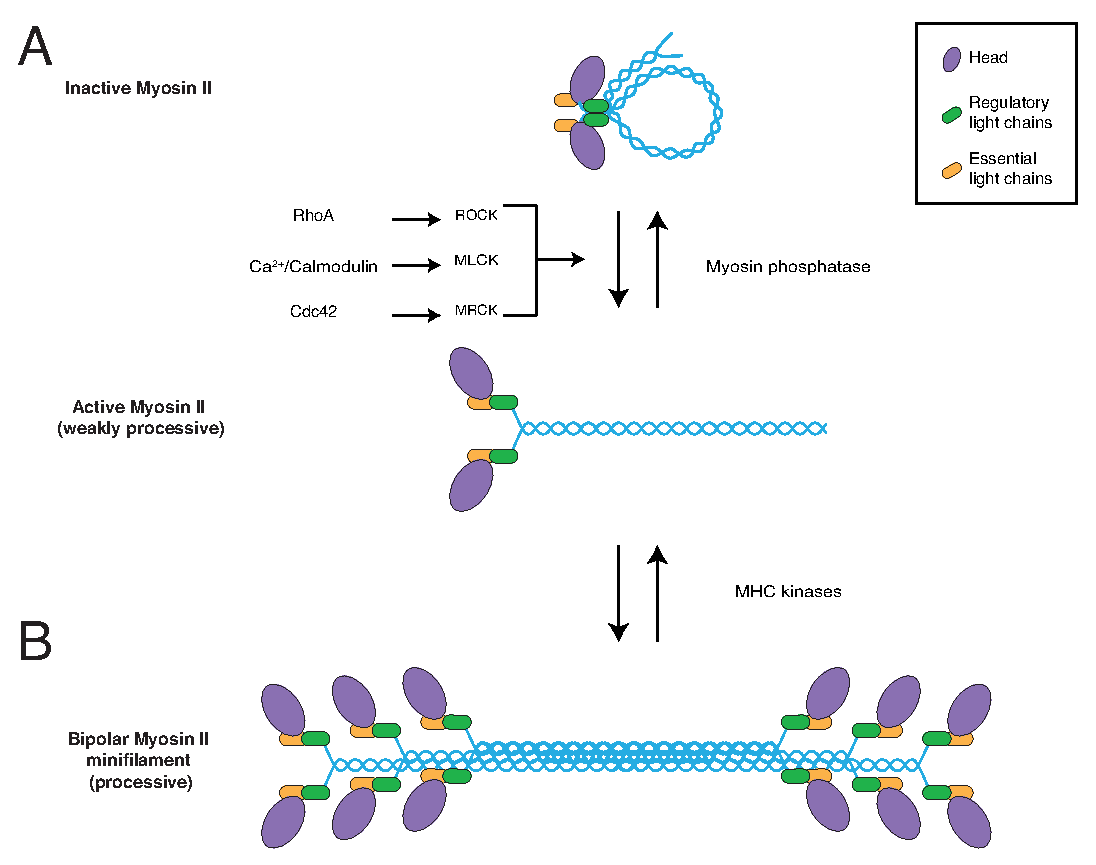
\includegraphics[width=1\textwidth]{Figure1-1}
\captionof{figure}[Structure and assembly of Myosin II minifilaments.]{\textbf{Structure and assembly of Myosin II minifilaments.} (A) When inactive, Myosin II adopts an inhibited folded conformation.  Myosin II is activated by phosphorylation of its regulatory light chain, which induces a conformational change. When active, Myosin II is unipolar and only weakly processive. (B) Phosphorylation of the Myosin II heavy chain controls the assembly of Myosin II into bipolar minifilaments.  In this state, Myosin II motors become highly processive.}
\end{figure}

%Introduction to non-muscle Myosin II (henceforth Myosin II)
 Non-muscle Myosin II is a ubiquitous class II myosin that is found in all eukaryotic cells \cite{Conti:2007hc, VicenteManzanares:2009ik}.  It has been shown to regulate cellular processes such as cell polarity, adhesion, and cell division.  Similar to myosin found in skeletal muscle tissue, non-muscle Myosin II is a hexamer that is highly processive when assembled into bipolar minifilaments.  Unlike skeletal muscle Myosin II, non-muscle Myosin II (henceforth myosin or Myosin II) minifilaments contain far fewer heads.  Based on calculations of the size and shape of minifilaments in their \textit{in vitro} assay, Niederman and Pollard estimated that Myosin II minifilaments derived from human platelet cells contain about 60 heads \cite{Niederman:1975uu}.

%Non-muscle Myosin II regulation
Myosin II activity is primarily regulated by the phosphorylation state of two highly conserved residues (serine 19 and threonine 18 in vertebrates) in the regulatory light chain (RLC) \cite{Moussavi:1993up}.  There are several kinases that have been shown to phosphorylate these residues both \textit{in vitro} and \textit{in vivo}.  These include myosin light chain kinase (MLCK), Rho-kinase (ROCK/Rok), and myotonic dystrophy-related Cdc-42 binding kinase (MLCK), all of which are controlled by members of the family of Rho GTPases \cite{Matsumura:2005cn}.  When the RLC is unphosphorylated, the mysoin II homodimer is autoinhibited by adopting a folded conformation that prevents F-actin binding, ATPase activity, and the formation of minifilaments (Figure 1.1A).  It was first observed in human platelet cells that phosphorylation of serine 19 was shown to significantly increase myosin's actin-dependent ATPase activity \cite{Adelstein:1975vn}.  It was also shown that phosphorylation of serine 19 allowed Myosin II to move actin filaments in \textit{in vitro} gliding assays \cite{Umemoto:1989tw}.  Phosphorylation of both serine 19 and threonine 18 increased enzymatic activity, but not actin filament gliding velocity \textit{in vitro}.  In the context of migrating fibroblasts, mono-phosphorylation of serine 19 promotes adhesion maturation, whereas di-phosphorylation promotes actomyosin bundling in the cell rear \cite{VicenteManzanares:2010gh}.  Phosphorylation of the regulatory light chain is also associated with relieving myosin autoinhibition.  Craig \textit{et al.} showed that phosphorylation of the light chain allows myosin to unfold and adopt an extended conformation (Figure 1.1A) \cite{Craig:1983tq}.  Furthermore, mono- and di-phosphorylation of the regulatory light chain also promoted the assembly of myosin into bipolar minifilaments (Figure 1.1B) \cite{Scholey:1980ui, Ikebe:1988uy}.  Although much less work has been done investigating the role of myosin heavy chain phosphorylation, there exists evidence that phosphorylation of the heavy chain is the major mode of myosin phospho-regulation in \textit{Dictyostelium} \cite{Heissler:2016fs}.


There are three Myosin II isoforms (Myosin IIA-C) in mammalian cells, all of which have different mechanochemistry properties.  While Myosin IIC is not as common, most cells contain Myosin IIA and Myosin IIB \cite{VicenteManzanares:2009ik}.  A detailed kinetic analysis performed by Kovacs \textit{et al.} revealed that the rate of ADP release for Myosin IIA is an order of magnitude greater than its rate of phosphate release \cite{Kovacs:2003ex}.  As a result, Myosin IIA has a low duty ratio that is comparable to that of skeletal muscle Myosin II.  In contrast, another study from the same group showed that the ratio of the rate of ADP release to the rate of phosphate release is much lower in Myosin IIB than that of Myosin IIA \cite{Wang:2003dq}.  Myosin IIB therefore has a higher duty ratio and is capable of exerting greater tension on actin filaments relative to Myosin IIA.  Furthermore, Myosin IIA and Myosin IIB have been shown to have different subcellular localization patterns \cite{Kolega:1998um}.  Combined, these results suggest that Myosin IIA and Myosin IIB might have different functions inside cells.  Indeed, a series of beautiful experiments by Vicente-Manzanares \textit{et al.} demonstrated that although Myosin IIA and Myosin IIB have some overlapping functions, they differentially regulate key aspects of cell migration such as adhesion maturation and rear formation \cite{VicenteManzanares:2007ep, VicenteManzanares:2008kj, VicenteManzanares:2011ha}.  




\subsection{Actin and actin-binding proteins} 
%Actin overview
Actin is a 42-kDa protein that is extremely abundant, highly conserved, and found in nearly all eukaryotic cells.  Like myosin, actin is an ATP binding protein that can assemble into higher order structures. Inside the cell, actin exists in two states: monomeric globular actin (G-actin) and filamentous actin (F-actin).  G-actin undergoes characteristic cycles of assembly into actin filaments, ATP hydrolysis, and disassembly of those filaments.  Actin monomers assemble into polar filaments containing dynamic barbed (plus) and relatively less dynamic pointed (minus) ends.  In filamentous form, actin is one of the major structural components of the cytoskeleton, and is responsible for maintaining cellular tension, generating protrusive forces, and providing tracks for intracellular transport.  The actin cytoskeleton is regulated by a host of nucleation, elongation, branching, capping, bundling, and severing proteins that give rise to rich dynamic properties \cite{Pollard:2016hj}.

%Figure 1.2
\begin{figure}[h!]
\centering
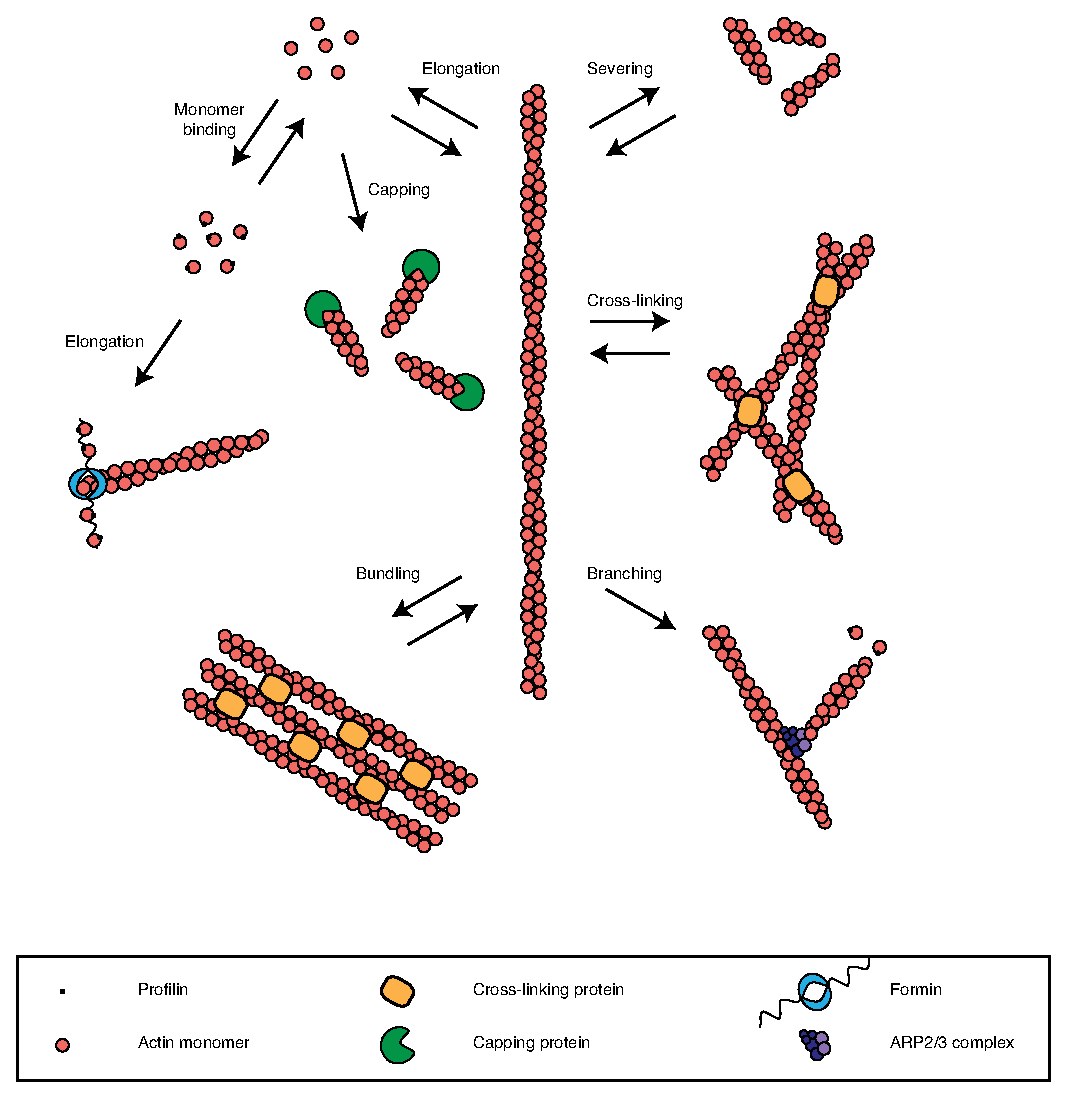
\includegraphics[width=1\textwidth]{Figure1-2}
\captionof{figure}[Overview of actin structures and actin binding proteins.]{\textbf{Overview of actin structures and actin binding proteins.} The structure and dynamics of actin networks is regulated by a host of actin binding proteins that bundle, branch, cross-link, sever, elongate, and cap actin filaments.}
\end{figure}


%Actin assembly and disassembly kinetics
Much of what we know about actin polymerization and depolymerization dynamics has come from \textit{in vitro} studies that monitored actin assembly and disassembly processes in sedimentation, fluorescence spectroscopy, and viscometry assays \cite{Pollard:2016hj}.  Actin polymerization is thought to occur in three sequential stages.  The first stage is the lag period, where actin monomers rapidly associate, often forming unstable oligomers.  Nucleation of actin dimers and trimers is thought to be the rate limiting step of actin polymerization \cite{Cooper:1983uk}.  Thus, the lag period appears to have a strong dependence on actin monomer concentration.  The second stage, which is the elongation stage, occurs when actin oligomers form a stable seed and rapidly elongate.  The third stage occurs when actin monomers and actin filaments have reached a steady state where there is no net polymerization.  The critical concentration of actin is the concentration of unassembled actin monomers in solution after the assembly assay reached steady state.  


%ATP hydrolysis and barbed end growth
Actin polymerization and depolymerization are driven by a complex ATP hydrolysis cycle.  Polymerization of actin filaments primarily occurs by addition of ATP-bound monomeric actin to the fast growing barbed end instead of the slow growing pointed end.  After a monomer has been added, ATP is rapidly hydrolyzed to ADP and inorganic phosphate.  Inorganic phosphate is then slowly released, resulting in ADP-F-actin.  During elongation, more ATP-bound monomers are added to the barbed while older subunits within the actin filament hydrolyze their ATP.  These older ADP-F-actin subunits are readily turned over by depolymerization and severing, and can then be recycled for later incorporation into other actin filaments and networks.


%Thymosin beta 4
The concentration of actin monomers within cells is much greater than the critical concentration required for the spontaneous polymerization of pure actin \textit{in vitro}.  At such high concentrations nearly all of the actin in a cell would be expected to be in filament form.  Instead, cells regulate actin polymerization through a host of actin binding proteins that function to promote or inhibit actin assembly.  One such protein is thymosin-$\beta$-4.  Thymosin-$\beta$-4 is currently thought to be the main actin-sequestering protein in cells \cite{Goldstein:2005kk}.  The concentration of thymosin-$\beta$-4 \textit{in vivo} has been shown to vary from 20$\mu$M in \textit{Xenopus} extracts to 600$\mu$M in platelets, which is at least twice the concentration of unpolymerized monomeric actin \cite{Pollard:2000bla}.  Thymosin-$\beta$-4 binds much more tightly to ATP-bound actin than ADP-bound actin.  When in complex, thymosin-$\beta$-4-bound G-actin cannot associate with the barbed or pointed ends of an actin filament.


%Profilin
Profilin, another actin monomer binding protein, was first characterized in spleen extracts as a small protein whose association with actin could explain actin's ability to persist as monomers under physiological conditions \cite{Carlsson:1977tv}.  Later experiments showed that Acanthamoeba profilin increased the critical concentration of Acanthamoeba actin \cite{Tseng:1982uc}.  Purified profilin was also shown to cause actin filaments at steady-state to depolymerize in a dose-dependent manner \cite{Tseng:1982uc}.  Together, these early results suggested that profilin functions to sequester actin monomers.  However, unlike thymosin-$\beta$-4, profilin is actually thought to promote actin filament assembly.  Indeed, profilin is able to promote addition of monomers selectively to the barbed ends of actin filaments without lowering the critical concentration \cite{Pring:1992us, Pollard:2000bla, Kang:1999wx}.  Furthermore, it has been shown that profilin-actin can be added to actin filament barbed ends with similar kinetics as actin monomers \cite{Kang:1999wx}.  This suggests that profilin maintains a large pool of actin monomers that would readily be incorporated into filaments by binding to any free barbed ends.

%Capping
Since actin filament elongation occurs rapidly at barbed ends, how do cells prevent the pool of actin monomers from being quickly depleted?  One way cells regulate their amount of free actin monomers is by regulating the number of free barbed ends through capping proteins.  It is thought that capping proteins are present at high enough concentrations, and with high enough affinity, to cap most barbed ends \textit{in vivo} \cite{Schafer:1996vi}.  Therefore, the coordinated behavior of capping proteins and actin monomer-binding proteins play an essential role in regulating the pool of actin monomers.


%Severing actin filaments
Cells use another protein known as ADF/Cofilin to regulate the concentration of actin monomers \cite{Hotulainen:2005im}.  ADF/Cofilin is an actin severing protein that is expressed in all eukaryotic cells, with mammalian cells containing three forms known as ADF, cofilin-1,and cofilin-2 \cite{Bernstein:2010cn}.  Cofilin-1,the major form of the protein found in non-muscle tissue, plays an important role in cytokinesis, cell migration, and cancer invasion \cite{Chen:2011jh, Roussos:2011kx}.  \textit{In vitro} studies have shown that low concentrations of cofilin promote actin depolymerization by severing actin filaments \cite{Andrianantoandro:2006hk}.  However, like other actin binding proteins, cofilin's function inside cells is highly complex and depends on its local concentration relative to other actin regulators \cite{Bernstein:2010cn}.  For example, cofilin-mediated severing can also promote actin polymerization by creating free barbed ends \cite{Ichetovkin:2002ur}.  This is important for the polymerization of branched actin networks in the lamellipodium during cell migration \cite{BravoCordero:2013ef}.  At very high concentrations, cofilin is thought to nucleate actin filaments directly \cite{Andrianantoandro:2006hk}.

%ARP-2/3 
Cells employ a variety of mechanisms such as actin-monomer binding, capping, and actin filament severing to prevent spontaneous nucleation of actin filaments.  Cells overcome these inhibitory functions through the use of various factors that catalyze the nucleation and elongation of actin filaments.  The ARP2/3 complex is one of the most abundant and well-understood actin nucleators.  It plays a role in processes such as cell migration, where it has been shown to create dendritic lamellar networks that propel the cell forward.  ARP2/3 was first purified based on its affinity for binding to profilin \cite{Machesky:1994wg}.  Unlike many other actin nucleators, ARP2/3 is unique because it nucleates branched actin filaments by binding to the side of pre-existing filaments.  ARP2/3 binds stably to the mother filament and nucleates a daughter 70$\,^{\circ}$ relative to the axis of the filament.  The ARP2/3 complex consists of seven subunits: ARP2, ARP3, and ARPC1-5 (actin-related protein complex) \cite{Goley:2006cr}.  ARP2 and ARP3 are structurally similar to actin, and also have ATP binding and hydrolysis activity.  ATP binding appears to be important for inducing large scale conformational changes that increase ARP2/3's affinity for nucleation promoting factors (NPFs).  The role of ATP hydrolysis by ARP2 remains unclear, as studies have linked ATP hydrolysis to nucleation and un-branching events \cite{Dayel:2004dy,LeClainche:2003bh}.  A cryo-EM structure of activate ARP2/3 complex suggests that the additional subunits might play a role in mediating contacts with the mother filament \cite{Egile:2005bm}.




%Regulation of ARP-2/3 
ARP2/3 by itself is not an efficient nucleator.  Three of the main regulators of ARP2/3 activity include binding to pre-existing actin filaments, phosphorylation of certain ARP2 (and \textit{maybe} ARP3) residues, and interactions with NPFs such as WAVE and WASP/SCAR \cite{Campellone:2010gd}.  The activity of these NPFs is in turn spatially and temporally regulated by various signal-transduction pathways \cite{Goley:2006cr}.  WASP (Wiskott— Aldrich syndrome protein) and WAVE (WASP-family verprolin-homologous protein) are class I NPFs that share a common WCA domain.  The WCA domain consists of a WASP-homology-2 (WH2) domain, a cofilin-homology (C) domain, and an acidic (A) domain.  The WH2 binds G-actin, while the CA (C and A domain together) region promotes ARP2/3 binding.  \textit{In vitro} studies have shown that the WCA domain is sufficient to activate AP2/3 to polymerize branched actin networks \cite{Goley:2006cr}.  It was originally thought that the WCA simply delivered an actin monomer to the ARP2/3 complex, thus promoting the formation of an actin trimer that can nucleate new branched filaments.  However, recent biochemical and structural studies suggest that the WCA domains of WAVE and WASP regulate a more complex mechanism where the CA domain induces a conformational change in ARP2/3 that brings ARP2 and ARP3 closer together while the WH2 domain delivers the actin monomer.

%Formin and unbranched networks
Unlike the ARP2/3 complex, all other known actin polymerization proteins form unbranched actin filaments.  The most common nucleators are ENA/VASP and formins.  Formins, found in nearly all eukaryotic cells, are both actin nucleators and elongators \cite{Chesarone:2010iw}.  Formins have been shown to build diverse cellular structures such as filopodia, stress fibers, yeast actin cables, and the cytokinetic ring \cite{Suarez:2016bw}.  Formin family proteins are characterized by the highly conserved formin homology domains FH1 and FH2.  Formins can be subdivided into different subclasses based on the divergence of the FH2 sequence \cite{Higgs:2005hn}.  However, sequence differences in the FH1 and FH2 domains of individual formins vary their ability to associate with actin filament barbed ends.  It is thought that these biochemical differences determine whether a a formin is better at nucleating or elongating actin filaments.

The domain organization of formins can be split into two groups: an N-terminal regulatory region that plays a role in localizing formins in vivo and auto-inhibiting its activity, and C-terminal active region that promotes actin filament assembly.  More specifically, the regulatory region of mammalian formins such as mDIA1-3 (similar to \textit{Drosophila} Diaphanous) contains a Rho GTPase-binding domain (GBD), a diaphanous inhibitory domain (DID), and a dimerization and/or coiled-coil domain (CC).  The active region of mammalian formins contains an FH1 domain, an FH2 domain, and diaphanous autoregulatory domain (DAD).  Formin functions as a dimer that changes conformation between an active and inactive state.  \texit{In vitro} experiments have shown that when formin is inactive, interactions between the DAD and DID domains inhibit actin polymerization by the FH2 domain.  In some instances this inhibition can be relieved by the binding of Rho GTPases near the DAD region.  The FH1 domain lacks a well-defined secondary structure, but contains a polyproline region that binds profilin.  The FH2 domain, which nucleates and elongates actin filaments, forms head-to-tail dimers that are topologically similar to a torus \cite{Xu:2004vc}.


%Formin nucleation and elongation
\textit{In vitro} experiments have shown that the FH2 domain is sufficient to nucleate actin filaments even though it has a low affinity for actin monomers  \cite{Pring:2003dw,Sagot:2002is}.  Instead, formin is thought to nucleate actin filaments by binding and stabilizing actin dimers \cite{Pring:2003dw}.  Therefore, the rate-limiting step for actin nucleation is the formation of short-lived actin dimers and trimers.  The FH2 domain does have a high affinity for actin filaments.  Once a stable filament is nucleated, actin can be elongated by formins.  An active formin will enclose the barbed end through interactions between the FH2 domain and the two terminal actin subunits.  These interactions between formin and barbed ends rely on proper dimerization of the FH2 domain.  Elongation then proceeds as formin processively caps and adds monomers to the barbed end.  The FH1 domain also plays a key role in filament elongation.  FH1-profilin interactions are thought to enhance actin filament elongation by increasing the local concentration of actin monomers near the barbed end \cite{Kovar:2006fm, Vavylonis:2006im, Paul:2008kv}.


\subsection{Rho GTPases: Master regulators of actomyosin contractility}
%Overview of Rho Regulating actin networks
The overall structure and contractile properties of actomyosin networks are determined by the regulation of myosin motor activity, the structure and density of the actin network, and the local concentrations actin binding proteins that cap, cross-link, bundle, and sever actin filaments.  Therefore, an unresolved challenge in cell biology is to understand how cells coordinate the activities of these overlapping sets of components in order to regulate the assembly of contractile networks in space and time.  Much research has shown that the Rho family of GTPases, a subfamily of the Ras superfamily, are important regulators of the actin cytoskeleton \cite{Hall:2012cg}.  Rho GTPases act as molecular switches to regulate a wide range of important cellular processes such as cytokinesis, vesicle trafficking, cell migration, and cell shape changes \cite{Piekny:2005dw,Symons:2003vy,Ridley:2001wu, EtienneManneville:2002fq}.  Classic work by Nobes and Hall was the first to demonstrate that the canonical Rho GTPase subclasses RhoA, Rac, and Cdc42 differentially regulate the formation of different actin structures within migrating fibroblasts \cite{Nobes:1995wn}.  They showed that RhoA stimulates the formation of stress fibers and focal adhesions, Rac promotes the formation of the lamellipodia, and Cdc42 promotes the formation of filopodia \cite{Nobes:1995wn}.  Since this discovery, Rho GTPases have been implicated in a diverse range of other processes such as adherens junction remodeling in \textit{Drosophila}, hyper-proliferation of cancer cells and metastatic tumor invasion \cite{Sahai:2002el}, and neurite growth during neuronal development \cite{Stankiewicz:2014bz}.



%Overview
Rho GTPases are monomeric proteins that are about 20kD in size \cite{Schaefer:2014ez}.  Like other GTPases, most Rho GTPases transition between an active conformation when bound to GTP and an inactive conformation when bound to GDP \cite{Hodge:2016cz}.  When active, Rho GTPases initiate signaling through interactions with a host of downstream effectors.  Biochemical studies have shown that Rho GTPases have a high affinity for guanine nucleotides, but intrinsically exchange GTP for GDP slowly \cite{Bos:2007cu}.  In addition, Rho GTPases also hydrolyze GTP slowly.  Therefore, the activity cycle of Rho GTPases is controlled to a large extent by three distinct classes of accessory proteins: GEFs, GAPs, and GDIs.  Guanine nucleotide exchange factors (GEFs) activate Rho GTPases by catalyzing the exchange of GDP for GTP.  They accelerate the rate exchange of GDP for GTP by several orders of magnitude \cite{Vetter:2001iw}.  GTPase activating proteins (GAPs) inactivate Rho GTPases by increasing their intrinsic ability to hydrolyze GTP.  Guanine nucleotide dissociation inhibitors (GDIs) prevent Rho GTPase activation and membrane localization by binding and sequestering the inactive GDP-bound conformation in the cytoplasm \cite{GarciaMata:2011hb}.  In addition, there exists certain post-translational modifications that further regulate the spatial and temporal activation of Rho GTPases \cite{Hodge:2016cz}.  For example, lipid modifications such as C-terminal prenylation localize Rho GTPases to specific membrane compartments. 


%Structure and function of RhoA domains
Along with Rac and Cdc42, RhoA is one of the most studied Rho GTPases.  Madaule and Axel inadvertently identified RhoA in the marine snail \textit{Alypsia} \cite{Madaule:1985wf}.  Since then, other isoforms of RhoA have been identified.  Structurally, RhoA consist of a G domain, a Rho insert region, and a C-terminal hypervariable region.  The G domain consists of five conserved motifs G1-G5.  The G1, G4, and G5 motifs are all involved in nucleotide binding, whereas the G2 and G3 motifs contain switch I and switch II regions, respectively.  The switch I and switch II regions interact with GAPs and GEFs, and change conformation depending on whether GDP or GTP is bound.  The insert region is located between the G4 and G5 regions, and functions to bind GEFs and downstream effectors proteins such as mDia and ROCK \cite{Lammers:2008gi, Zong:2001ho}.  Phosphorylation of the C-terminal hypervariable region appears to play a role in RhoA inactivation by promoting GDI binding and membrane dissociation \cite{Clague:2012gb}.  Next to the hypervariable region, the C-terminus contains a CAAX-box that can be posttranslationally modified by attachment of a lipid anchor.  The lipid anchor plays a role in subcellular localization as well as GDI binding. 




%Short Paragraph on GAPs and GEFs (Upstream)
The activity of RhoA is also determined by the balance between its activators (GEFs) and its inhibitors (GAPs).  There are over 70 different Rho GEFs and about 80 different Rho GAPs in mammals \cite{Cherfils:2013ks}.  GEFs can be classified into two different families, either DBL or DOCK, based on their structure.  DBL-family GEFs are the largest and best understand Rho GEFs \cite{Rossman:2005do}.  They are characterized by a DBL-homology (DH) domain that is associated with a pleckstrin homology (PH) domain.  The DH domain interacts with the switch regions of RhoA to catalyze the exchange of GDP for GTP \cite{Rossman:2005do}.  Variable interactions between the poorly conserved switch-back region of the DH domain and the G domain of RhoA mediates DBL GEF selectivity amongst Rho isoforms \cite{Rossman:2005do, Schaefer:2014ez}.  Like GEF activation, GAP inactivation of RhoA is mediated by interactions with the switch regions \cite{Cherfils:2013ks}.  However, much less is known about how Rho GAPs differentiate between the different Rho isoforms.  The large number of GAPs and GEFs, as well as the variations in their binding and catalytic regions, enumerate the myriad biochemical pathways that RhoA controls \cite{Schaefer:2014ez}.  


%Rho Downstream effectors: ROCK and Dia/%Organization of cortical actomyos
The specific activation, localization, and signalling of RhoA provides a basis for the selective activation and recruitment of specific downstream effector proteins in different cellular contexts.  It is through these effector proteins that RhoA can promote the formation of distinct actomyosin structures.  One important and well-studied example is the assembly and constriction of the contractile ring during cytokinesis.  Cytokinesis involves properly positioning the site of furrow ingression, recruiting factors that promote actin and myosin II assembly into an actomyosin ring, and constricting the membrane to form two daughter cells.  RhoA regulates this complex process by promoting actin filament polymerization and myosin II mini-filament assembly through formin and Rho kinase, respectively.  RhoA has also been shown to recruit the scaffold protein anillin, which might function to stabilize myosin II in the contractile ring \cite{Piekny:2008jf}.  Although there are multiple Rho GTPases involved in cytokinesis, RhoA seems to be the most important \cite{Piekny:2005dw}.  Indeed, RhoA localizes to the furrow independent of actin and myosin, and inhibiting RhoA activity prevents furrow ingression in many different animal cells  \cite{Yuce:2005hz, Piekny:2005dw}.  Furthermore, an important recent study by Wagner and Glotzer showed that local photo-activation of RhoA is sufficient to induce furrow formation \cite{Wagner:2016ev}.  


\section{Review of pulsed contractility}
\subsection{Pulsed contractions are ubiquitous}
%Broad overview of what pulsed contractions are (maybe include a figure)
Pulsed contractility is a common mode of contractility that has been observed in a wide range of contexts.  Pulsed contractions are characterized by cycles of actin assembly and myosin activation, local force generation that transiently deforms cellular surfaces, and disassembly.  Although pulsed contractions were first identified in the early \textit{C. Elegans} embryo, much of what we know about the mechanisms underlying pulsed contractions comes from studies of epithelial morphogenesis during early \textit{Drosophila} development.  During gastrulation, pulsed contractions are thought to play a key role in promoting tissue bending and elongation.  In this section, I review what is currently known about how pulsed contractions drive during mesoderm invagination and germ band elongation in \textit{Drosophila}.


\subsection{Pulsed contractions in \textit{Drosophila} Mesoderm invagination}
%Introduction to Mesoderm invagination
Mesoderm invagination is one of the first steps of \texit{Drosophila} gastrulation.  Early work showed that two transcription factors, \textit{snail} and \textit{twist}, are required for proper development of the mesoderm \cite{Simpson:1983wv}.  In a later study, Leptin and Grunewald made the key observation that both \textit{snail} and \textit{twist} are expressed in the ventral cells in the presumptive mesoderm \cite{Leptin:1990ub}.  They also provided a detailed description of the cell shape changes that occur during mesoderm invagination \cite{Leptin:1990ub}.  Mesoderm invagination can be thought of as a two-step process.  During the first step, ventral cells apically constrict and bend the tissue to form a ventral furrow.  During the second step, the presumptive mesoderm cells spread out under the ectoderm to form the second germ layer.  



%Apical constriction 
Apical constriction is a common cell shape change that occurs in many organisms and during many stages of embryogenesis \cite{Sawyer:2010ku}.  By shrinking its apical surface, a columnar, or cuboidal, epithelial cell can adopt a wedge-shaped geometry that can promote different tissue architectures depending on the developmental context \cite{Martin:2014bi}.  If cells maintain adhesive contacts, coordinated apical constriction can promote bending, folding, and invagination of epithelial tissues.  Apical constriction can also promote cell ingression, extrusion of apoptotic cells, and wound healing \cite{Martin:2014bi}.  Apical constriction was first thought to proceed through a purse-string mechanism, where cell surface deformation is driven by circumferential actin and Myosin II continuously contracting and exerting force on adherens junctions \cite{Lecuit:2007cw}.  This mechanism has been supported by classic studies on \textit{Xenopus} neurulation \cite{Martin:2014bi}.  However, there is also growing evidence that dynamic actomyosin networks on the apical cortex can drive apical constriction \cite{Martin:2014bi,Davidson:2012bf}.  

%Martin et al 2010
Martin \textit{et al.} demonstrated that apical constriction of \textit{Drosophila} ventral cells is not driven by a purse-string mechanism \cite{Martin:2009du}.  Instead, pulsatile contractions of the medioapical cortex shrink the apical surface of ventral cells in a two step ratchet-like manner \cite{Martin:2009du}.  During the first step, known as the constriction phase, a decrease in apical surface area is strongly correlated with a large increase in the constriction rate.  The second step is a stabilization phase, where the previously reduced apical surface area remains constant in the absence of any constriction.  By imaging live cells expressing fluorescent markers for the membrane and Myosin II, they assayed myosin dynamics during apical constriction.  During the constriction phase, the authors observed that pulsed accumulation and coalescence of myosin punctae was also strongly correlated with a decrease in apical surface area.  The accumulation of myosin to the apical surface was mostly medial, and its coalescence into pulses required an intact medioapical actin meshwork.  They also observed a strong correlation between the accumulation rate of myosin and the constriction rate.  The myosin foci then disappeared during the stabilization phase.  

Martin \textit{et al.} confirmed that this two step apical constriction process is under the control of the transcription factors \textit{snail} and \textit{twist} \cite{Martin:2009du}.  They observed that Myosin II pulses did not form in the absence of \textit{snail}, and that ventral cells did not decrease their apical surface area.  In the absence of \textit{twist},  Myosin II  did not localize medioapically, but instead accumulated to the junctions.  The ectopic accumulation of Myosin II to the junctions was associated with transient decreases in cell surface area that were not stabilized.  These results suggest that \textit{snail} is required for the constriction phase, while \textit{twist} is required for the stabilization phase.

In order for ventral furrow cells to decrease their apical surface area through a pulsatile mechanism, contractile actomyosin pulses must transmit forces across adherens junctions.  Furthermore, an intact apical actomyosin network is required to maintain the transient cell shape changes the occur during the stabilization phase between pulses.  How, then, are these apical actomyosin networks assembled and regulated during ventral furrow invagination?  How are apical actomyosin dynamics and adherens junction remodeling coupled?

In a subsequent paper from the Martin group, Mason \textit{et al.} addressed these questions by focusing primarily on factors downstream of Twist activity, namely the GTPase RhoA (Rho1 in \textit{Drosophila}) and its effectors Rok and Dia \cite{Mason:2013ee}.  The authors showed that RhoA, Rok, Myosin II, and Dia all co-localize medioapically in ventral furrow cells \cite{Mason:2013ee}.  They also showed that RhoA, Dia, F-actin, and E-cadherin co-localize in the junctional domains.  Rok activity is required for the proper localization and activation of Myosin II to the apical surface of ventral furrow cells.  The authors confirmed this by inhibiting Rok activity with the Rho kinase inhibitor Y-27632.  Under these conditions, there was  Myosin II no longer formed pulses.  As expected, the loss of myosin pulses prevented the decrease in apical surface area of ventral furrow cells.  Rok activity was also shown to be required for condensing the actin cables that span the apical surface.  These results are consistent with Rok activity being necessary for stabilizing Myosin II pulses and shape changes following pulses.  However, Rok activity is not required  to assemble the medioapical actin network.  Instead, the medioapical actin network is mediated by the formin Dia.  In addition to building the apical actomyosin meshwork, Dia-mediated F-actin polymerization also regulates the localization of E-cadherin.  Indeed, the presence of a partial loss-of-function $\textit{dia}^M$, the authors showed that E-cadherin no longer localized to junctions, but instead localized across the apical surface.

%Paragraph about Twist and snail
How, then, do Twist and Snail coordinate Rok activity, F-actin network assembly and architecture, and E-cadherin dynamics even though these factors localize to separate domains?  The authors demonstrated that Twist and Snail play distinct roles in regulating both F-actin and Rok.  For example, \textit{snail} mutants lack a medioapical actin network as well as junctional F-actin cables.  In addition, in \textit{snail} mutants Rok and Myosin II localize to the subapical junctions instead of the apical surface.  In contrast, \textit{twist} mutants fail to form actin cables that span the apical cortex, and instead form a punctate medioapical actin network.  Furthermore, Rok and Myosin II localize to apical junctions in \textit{twist} mutants.  These observations are consistent with previous work showing \textit{twist} mutants undergoing cycles of pulsatile cell shape change that are not stabilized \cite{Martin:2009du}.  Together, these results suggest a mechanism where Twist spatially and temporally coordinates Myosin II activity, F-actin assembly and junctional remodeling by mediating differential localization of Rok/Myosin II and E-cadherin.  The authors propose that Twist does this by polarizing RhoA activity in the plane of the apical surface.





\subsection{Pulsed contractions in \textit{Drosophila} Germ band elongation}
%Introduction to germ band elongation and cell intercalation in Drosophila 
Germ band extension is a morphological process that gives rise to the thorax and abdomen in \textit{Drosophila}.  Germ band extension starts shortly after the beginning of gastrulation.   Similar to other systems such as \textit{Xenopus} convergent extension and chick neurulation, cellular rearrangements during \textit{Drosophila} germ band extension are mostly driven by cell intercalation \cite{Irvine:1994ug}.  In the \textit{Drosophila} germ band, cells intercalate along the dorsoventral axis.  Other cell shape changes and oriented cell divisions are only thought to contribute a small amount to elongating the tissue \cite{daSilva:2007er}.  One of the hallmarks of germ band extension is the extensive remodelling of adherens junctions between neighboring cells \cite{Bertet:2004ch}.  First, the 'vertical' junctions parallel to the dorso-ventral axis are shortened.  Then, germ band cells transition from having ‘vertical’ type 1 junctions that are perpendicular to the anterior-posterior axis, to having ‘horizontal’ type 3 junctions which are perpendicular to the old type 1 junctions and oriented along the anterior-posterior axis \cite{Bertet:2004ch}.  As a result of these junctional shrinkages, the germ band doubles in length along the anterior-posterior axis, and decreases in width along the dorsoventral axis.


%Pulsed contractions: Rauzzi paper
How are the junctions in the ectoderm remodeled during germ band elongation?  One reasonable hypothesis is that junctional accumulation of Myosin II drives junction shrinkage during cell intercalation.  Indeed, Bertet \textit{et al.} showed that the Myosin II heavy chain (Zip in \textit{Drosophila}) localizes to apical junctions only in the intercalating cells \cite{Bertet:2004ch}.  They also showed cell intercalation was severely disrupted in \textit{zip} mutants \cite{Bertet:2004ch}.  They observed that junctional modeling did not occur in \textit{zip} mutants, and that type 1 junctions persisted without changing  \cite{Bertet:2004ch}.  The authors sought to corroborate these results by inhibiting Rok activity with the Rho kinase inhibitor Y-27632.  They observed a decrease in Myosin II localization to the junctions in the absence of Rok activity.  Similar to the \textit{zip} mutant, embryos treated with Y-27632 showed severe defects in cell intercalation and junctional remodeling.  Laser ablation experiments by Rauzi \textit{et al.} demonstrated that the vertical junctions are under tension \cite{Rauzi:2008gz}.  Taken together, these results support the idea that planar polarized Myosin II contractility shrink the vertical dorsoventral junctions by increasing junctional tension.

However, Rauzi \textit{et al.} used improved imaging techniques and statistical analysis to reveal an alternate mechanism driving cell intercalation in the \textit{Drosophila} germ band \cite{Rauzi:2010fs}.  By imaging embryos expressing the Myosin II regulatory light chain (MRLC, Sqh in \textit{Drosophila}) fused to GFP, they identified two pulsating pools of Myosin II: one junctional and one medial.  Interestingly, the medial pool of Myosin II (along with F-actin) coalesces into pulses reminiscent of pulsed contractions in ventral furrow cells \cite{Martin:2009du}.  However, one key difference is that Myosin II pulses in ventral furrow cells form medially, while Myosin II pulses in germ band cells form near the junctions \cite{Martin:2009du, Rauzi:2010fs}.  They observed that there is a strong correlation between the formation of medial and junctional pulses, with medial pulses forming $\sim$8 seconds before junctional pulses \cite{Rauzi:2010fs}.  Similarly, they observed Myosin II contractions occurred in the medial region $\sim$10 seconds before they occurred in the junctional region \cite{Rauzi:2010fs}.  Each round of contraction correlated with a stepwise decrease in junction length \cite{Rauzi:2010fs}.  Surprisingly, by ablating medial Myosin II pulses near junctions, the authors showed that medial Myosin II pulses cause junction shrinkage \cite{Rauzi:2010fs}.  Furthermore, they observed that junctional shrinkage only occurs when junctional pulses follow medial pulses.  Therefore, the authors suggest a mechanism in which junctional pulses stabilize shortened junctions that have been shrunk by medial pulses \cite{Rauzi:2010fs}.  Similar to apical constriction in ventral furrow cells, the pulsed contractions that drive junctional shrinkage in the germ band depend on local activation of RhoA \cite{Mason:2013ee, Munjal:2015bx}.



\section{Pulsed contractions are an excitable system}
The main goal of this thesis is to understand the mechanisms underlying the initiation and termination of pulsed contractions.  At the molecular scale, this requires gaining insight into how cells regulates the activation/deactivation, assembly/disassembly, and mobility of actomyosin and various regulatory factors in space and time.  Based on the dynamics of Myosin II appearance and disappearance within pulsed contractions, we hypothesize that pulsed contractions are an excitable system (Figure 1.3 and Figure 1.4).  In general, excitable systems are characterized by fast positive feedback that rapidly turns activity on, and delayed negative feedback that turns it back off.  Excitable phenomena are common in nature, and include common processes such as action potentials, calcium spikes, and various modes of gene and hormone regulation \cite{Izhikevich:2007aa, Goldbeter:1996aa, Strogatz:1994tz}.  Recent work has demonstrated that actomyosin networks can also behave as excitable systems that have the capacity to form a rich multitude of complex spatial patterns such as pulses, oscillations, and traveling waves \cite{Ryan:2012bq, Allard:2013if, Dierkes:2014tm}.

%Figure 1.3
\begin{figure}[!htbp]
\centering
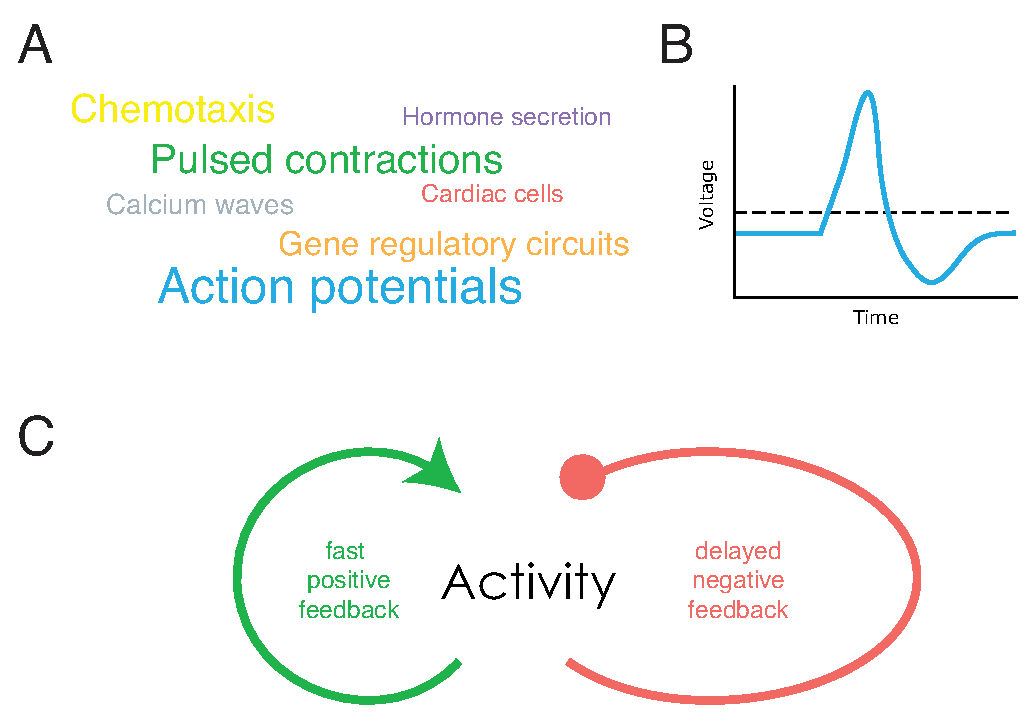
\includegraphics[width=1\textwidth]{Figure1-3}
\captionof{figure}[Pulsed contractions are an excitable system.]{\textbf{Pulsed contractions are an excitable system.} (A) Word cloud of well-known biological phenomena that are thought exhibit excitable dynamics. (B) Example of an action potential. (C) Simple feedback circuit diagram illustrating the two key requirements for excitable dynamics: fast positive feedback and delayed negative feedack.}
\end{figure}




\subsection{Contractile Instability Model}
%Introduction the contractile instability model, Turing, Meinhardt
The mathematical analysis of spontaneous pattern formation during morphogenesis has been extensively studied since Alan Turing published his seminal paper in 1952 \cite{Turing:1952vn, Kondo:2010bx}.  Turing proposed that a system of morphogens that are reacting and diffusing  is sufficient to drive spatial patterning within biological tissues.  His key insight was that diffusion could destabilize the steady state of a system of reacting chemicals.  This insight was counterintuitive, as diffusion can be thought to dampen spatial heterogeneities.  In the paper, Turing described a reaction-diffusion mechanism in which an activator species diffused slowly, while an inhibitor species diffused more rapidly.  Based on their differential diffusivities, and mutual interactions, Turing showed that a small spatial perturbation can destabilize the activator-inhibitor system at steady state.  The small perturbation is amplified over time, leading to a new steady state where the concentration of each species varies with position.  This mechanism is an example of diffusion-driven instability \cite{Segel:1972wb}.

Gierer and Meinhardt, and independently Segel and Jackson, extended Turing's reaction-diffusion system of morphogens into a more general class of models \cite{Gierer:1972vq,Segel:1972wb}.  Their mathematical analysis confirmed that there are two features that play a central role in pattern formation: \textit{local autocatalytic activation of the activator} and \textit{long-range inhibition by the inhibitor}.  The activator is autocatalytic if a small increase in its concentration/activity promotes a further increase in concentration/activity.  In general, the autocatalysis does not have to be direct and could instead be mediated by other factors that have been abstracted away in the model.  Autocatalysis alone is not sufficient to generate spatial patterns. Once the activator starts to increase, positive feedback would lead to global activation.  Thus in order for spatial patterns to form, autocatalysis of the activator must be modulated by long-range inhibition by a rapidly-diffusing inhibitor.  


%Figure 1.4
\begin{figure}[!htbp]
\centering
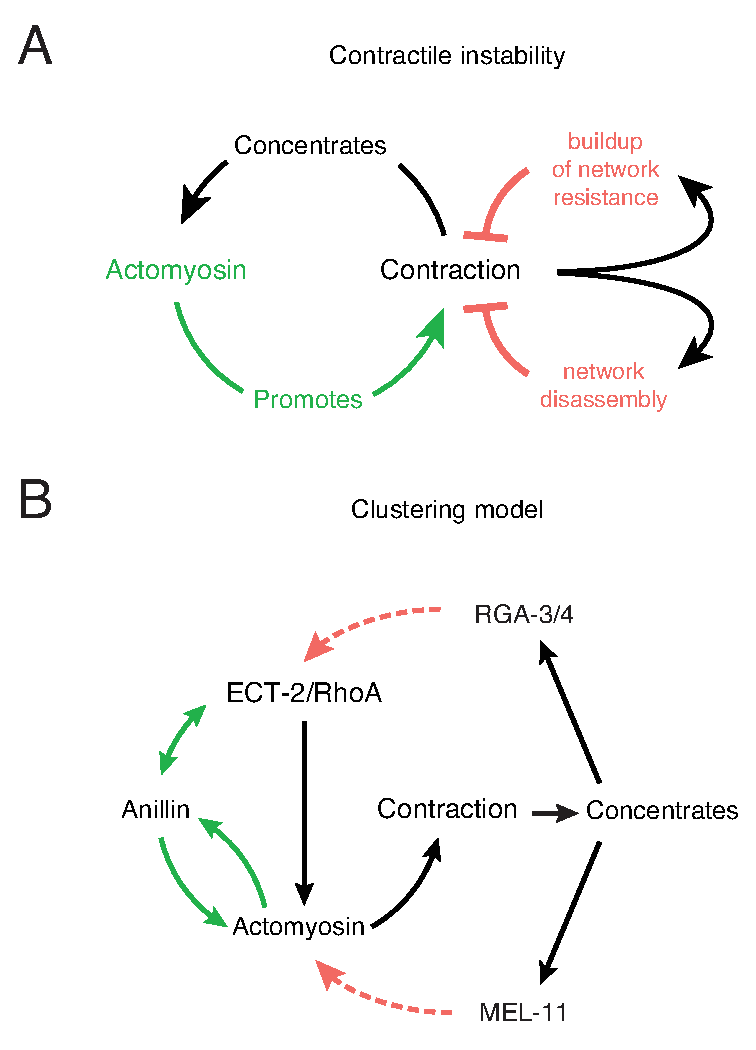
\includegraphics[width=0.85\textwidth]{Figure1-4}
\captionof{figure}[Potential feedback mechanisms governing the initiation and termination of pulsed contractions.]{\textbf{Potential feedback mechanisms governing the initiation and termination of pulsed contractions.} (A) \textbf{Contractile instability model:} Local Myosin II contractility concentrates F-actin, Myosin II, and/or their upstream regulators.  Network disassembly or a build up of network resistance can negatively feedback to inhibit contractility. (B) \textbf{Clustering model:} Anillin-mediated positive feedback clusters contractile components by mediating mutual binding interactions between F-actin, Myosin II, and or ECT-2/RhoA.  Delayed inhibition of RhoA or Myosin II is one potential form of delayed negative feedback in the system.}
\end{figure}



Although Turing noted the importance of mechanics in morphogenesis, his reaction-diffusion model did not take into account the mechanical properties of living tissues \cite{Howard:2011da}.  We now know that forces generated by the actomyosin cytoskeleton play an important role in tissue morphogenesis.  In terms of mechanical properties, the cytoskeleton can be thought of as an active fluid \cite{Kruse:2004il}.  Actomyosin networks continually consume energy, and have fluid-like properties that depend on the length, stability, and cross-linking of actin filaments \cite{Kruse:2004il}.  Bois \textit{et al.} developed a mathematical model of pattern formation of the cortex in which they model the cytoskeleton as an active fluid \cite{Kruse:2004il, Bois:2011kx}.  Although their mathematical analysis was similar to that of Turing and others, Bois \textit{et al.} departed conceptually from older models by considering advection-driven instability \cite{Turing:1952vn,Gierer:1972vq,Segel:1972wb,Bois:2011kx}.  They showed analytically that a single chemical species that obeys certain reaction-diffusion-advection equations is capable of generating spatial patterns.  In their model, it is essential that local force generation is proportional to the concentration of the chemical species.  As a result, their model recapitulates the local activation and lateral inhibition properties proposed by Gierer and Meinhardt \cite{Gierer:1972vq}.  Positive feedback in this model occurs when a local increase in the concentration of the activator promotes a further increase in concentration due to advection (Figure 1.4A).  Lateral inhibition occurs when neighboring regions of the cortex are depleted of the activator.  Interestingly, Bois \textit{et al.} showed that their model is capable of generating patterns in the absence of chemical reactions \cite{Bois:2011kx}.  Later work from the same group showed that by including reaction terms, their simulations could generate pulsatile patterns that are reminiscent of Myosin II pulses observed animal cells \cite{Kumar:2014ux, Munro:2004jk}.  Simulations from the Munro lab suggest that network disassembly, or a build up of network resistance, can provide delayed negative feedback in terminating pulsed contractions (personal communication).


%\subsection{Tension-based myosin accumulation}


\subsection{Clustering Models}
Another model that could explain pulsed contractility is a clustering model in which a scaffold protein promotes the accumulation of factors important for pulsed contractions.  Anillin is a scaffold protein that was first identified as an F-actin bundling protein in \textit{Drosophila} \cite{Miller:1989vn}.  Later work showed that Anillin also binds Myosin II \cite{Piekny:2010es,Zhang:2010fb}.  In the most general form of the clustering model, Anillin could promote pulsed contractions by mediating mutual interactions between factors such as RhoA, Ect2, Myosin II, and F-actin.   Maddox \textit{et al.} proposed a similar model to explain pulsed contractions in the early \textit{C.elegans} embryo \cite{Maddox:2005gd}.  Under wild-type conditions, \textit{C.elegans} embryos exhibit membrane ruffling in which deep membrane invaginations correspond to pulsed contractions (\cite{Maddox:2005gd}, see Chapter 2).  Maddox \textit{et al.} showed that \textit{C.elegans} embryos that have been strongly depleted of Anillin fail to ruffle \cite{Maddox:2005gd}.  They also showed that Myosin II failed to accumulate robustly in cortical patches when Anillin was depleted \cite{Maddox:2005gd}.  Instead, Myosin II localized uniformly on the cortex.  Furthermore, Anillin formed cortical patches that appeared to have roughly the same size in spacing as wild-type patches in the absence of Myosin II \cite{Maddox:2005gd}.  Maddox \textit{et al.} proposed a model in which local clusters of anillin, independent of Myosin II-dependent contractility, promote pulsed contractions by locally recruiting F-actin and Myosin II.  In this model, positive feedback between anillin and F-actin drives the accumulation of other factors such as Myosin II and septin.


%Anillin could mediates RhoA recruitment
In an alternate clustering model, Anillin-mediated autocatalytic activation of RhoA could recruit Myosin II and F-actin to pulsed contractions (Figure 1.4B).  Piekny \textit{et al.} provided evidence that suggested that RhoA and Anillin might regulate each other's localization to the cytokinetic furrow in dividing HeLa cells \cite{Piekny:2008jf}.  They showed that Anillin failed to localize to the furrow in the absence of RhoA, and that Anillin stabilizes RhoA in fixed cells \cite{Piekny:2008jf}.  They also showed that human Anillin contains a conserved C-terminal domain (called the Anillin homology domain) that is required for Anillin to function and localize properly \cite{Piekny:2008jf}.  They also showed that the Anillin homology domain binds active RhoA.  Later work by Frenette \textit{et al.} showed that the Anillin homology domain interacts with the PH domain of human Ect2 during cytokinesis \cite{Frenette:2012do}.  Furthermore, recent work by Manukyan \textit{et al.} showed that overexpressing Anillin in HeLa cells leads to an increase in RhoA activation \cite{Manukyan:2015gg}.  Taken together, these results suggest a mechanism whereby Anillin could promote autocatalytic activation of RhoA, and hence pulsed contractions, by locally mediating interactions between RhoA and Ect2 on the cortex.  


Since Anillin is a scaffold protein, it could mediate the initiation of pulsed contractions through multiple parallel pathways.  For example, in addition to promoting RhoA auto-activation, Anillin  could also promote contractile instability by stabilizing interactions between Myosin II and F-actin.  Support for this model comes from experiments where Piekney \textit{et al.} showed that Anillin stabilizes Myosin II at the furrow during cytokinesis \cite{Piekny:2008jf}.  Furthermore, Maddox \textit{et al.} showed that although depletion of Anillin led to a strong decrease in the amplitude and duration of Myosin II pulses in \textit{C.elegans} embryos, weak Myosin II pulses still formed on the cortex.



\section{My work}
%Pulsed contractions are ubiquitous
Much of what we know about how pulsed contractions are regulated, and what we can surmise about their functional importance, has come from studies in \textit{Drosophila} where they have been implicated in tissue invagination, tissue elongation, tissue closure, and wound healing \cite{Martin:2009du,Rauzi:2010fs, Solon:2009hg, Razzell:2014eb}.   However, pulsed contractions have also been documented in other organisms.  For example, early studies have documented pulsed contractions during polarization in early \textit{C. elegans} embryos and convergence extension in \textit{Xenopus}  \cite{Munro:2004jk, He:2010gf}.  More recent studies have shown that pulsed contractions might also play an important role in driving shape changes during compaction in mouse embryos, as well as apical constriction during neural tube closure in \textit{Xenopus} \cite{Maitre:2015hc, Christodoulou:2015kb}. 

%Why study pulsed contractions
The fact that pulsed contractions are ubiquitous in higher eukaryotes suggests that they likely play important functional roles, even though those roles may not be immediately apparent.  One possibility is that pulsed contractions might provide a way for cells within tissues to rapidly sample different conformations as they change shape.  Another possibility is that pulsed contractions help to maintain tissue integrity during morphogenesis \cite{Vasquez:2014hv}.  For example, since apical constriction of ventral furrow cells is asynchronous, pulsatile shape changes might reduce tension within the tissue \cite{Martin:2009du, Vasquez:2014hv,Fischer:2014hm}.  Thus future experimental or theoretical studies might provide insight as to why \textit{Drosophila} embryos, for example, might prefer pulsed contractions over circumferential actin cables for driving apical constriction.  From a more general perspective, pulsed contractions might belong to a broader class of mechanisms that include phenomena such as cell shape oscillations and wound healing \cite{Gorfinkiel:2016bv,Razzell:2014eb}.  From a more basic perspective, pulsed contractions are an interesting example of a complex self-organized contractile system.  Therefore, studying pulsed contractions might provide insight into the principles governing the assembly of actomyosin networks, as well as uncover general mechanisms that cells use to tune actomyosin networks to accomplish specific tasks.


%Outline my approach
How, then, are pulsed contractions initiated and terminated?  Which factors are required for pulsed contractions?  In what order are these factors recruited to pulsed contractions?  What determines the size and spatial organization pulsed contractions?  How might different organisms tune the activity of regulatory molecules and the assembly/disassembly kinetics of actomyosin in order to regulate the dynamics of pulsed contractions?  Previous experimental and theoretical research has given us a roadmap for answering these questions.  Building on these previous results, the purpose of this thesis is to provide insight into some of the unanswered questions, as well as provide a novel conceptual framework for guiding future experiments.  In the remainder of this chapter I will outline my general approach and provide a preview of chapters 2 and 3.  First, I will provide the rationale for using \textit{C. elegans} as a model system for pulsed contractility and introduce the relevant components.  Next, I will describe the experimental and modeling approach that my collaborators and I have taken to investigating pulsed contractions.  Last, I will describe the significance of the work we have done.


\subsection{\textit{C. elegans} as a model system for studying pulsed contractions}
Pulsed contractions were first identified in the \textit{C. elegans} where they occur during polarization in the zygote P0, during the first cell division, in the larger anterior daughter cell AB, and at the first stage of gastrulation (Figure 1.5) \cite{Munro:2004jk, RohJohnson:2012cf}.  Preliminary observations also suggest that pulsed contractions occur in the smaller posterior daughter cell P1 after the first cell division (data not shown).  Although we currently suspect that pulsed contractions do not play a significant functional role in \textit{C. elegans} development, there are many reasons that make the early embryo an excellent system to study actomyosin dynamics in general, and pulsed contractions in particular.  First, \textit{C. elegans} has a rapid generation time and is very easily cultured \cite{Jorgensen:2002ej}.  Second, the \textit{C. elegans} early embryo is large and optically clear, and the availability of many fluorescent markers makes it easy to acquire high quality images of the cortex with high spatial and temporal resolution.  Third, pulsed contractions in \textit{C. elegans} occur in both the single cell zygote P0 and the larger anterior daughter cell AB in the two cell stage (Figure 1.5).  P0 and AB are both large single cells, and the pulses are highly stereotyped within each context.  We can therefore compare and contrast pulses in P0 to pulses in AB in a quantitative manner by making reproducible measurements that have statistical significance.  For example, we can use cutting edge single-molecule techniques to measure the turnover and mobility of various components of the cortex \cite{Robin:2014jf}. 

%Figure 1.5
\begin{figure}[!htbp]
\centering
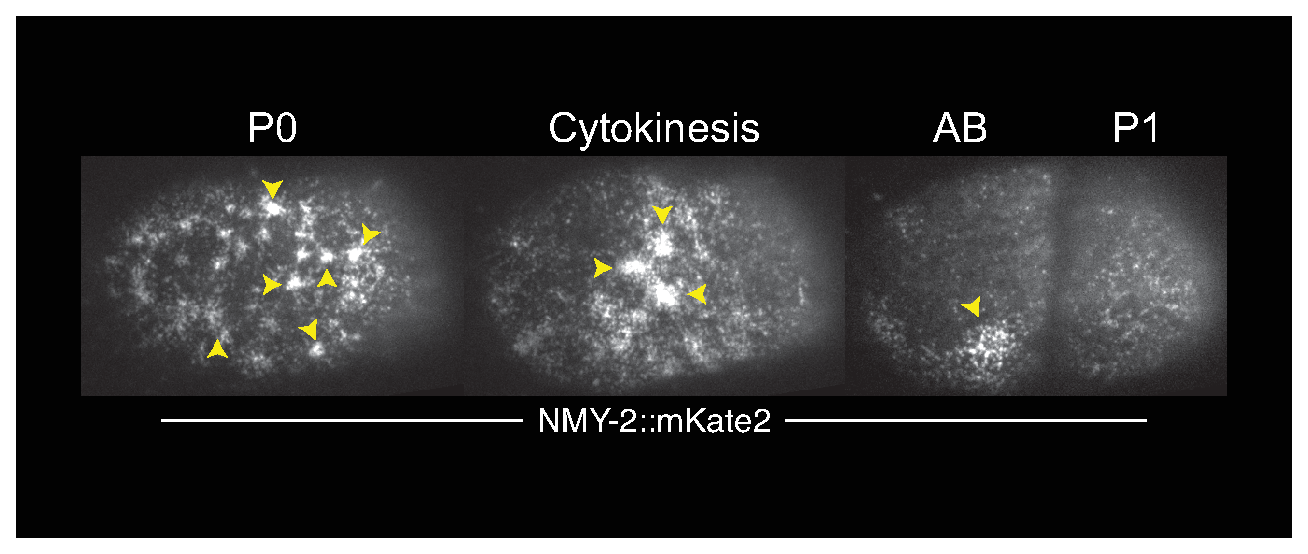
\includegraphics[width=0.85\textwidth]{Figure1-5}
\captionof{figure}[Pulsed contractions in the early \textit{C.elegans} embryo.]{\textbf{Pulsed contractions in the early \textit{C.elegans} embryo.} Micrographs of a representative \textit{C.elegans} embryo expressing NMY-2::mKate2 during the 1-cell stage, cytokinesis, and 2-cell stage.  Yellow arrowheads indicate pulsed contractions.}
\end{figure}

%Genetics as a tool
Another compelling reason for using the \textit{C. elegans} embryo as a model system is due to its history as a classic model organism.  As such, we know a great deal about \textit{C. elegans} genetics \cite{Jorgensen:2002ej}.  Large-scale mutagenesis screens, like the original screen by Sydney Brenner, have identified numerous mutant phenotypes \cite{Brenner:1974wn}.  Similarly, RNA interference (RNAi), either by feeding or injection, has also been used to conduct large-scale screens \cite{Timmons:2001wg, Kamath:2003bk}.  A recent RNAi  screen by Fietvet \textit{et al.} has identified important regulators of cell polarity and actomyosin contractility in \textit{C. elegans} \cite{Fievet:2013ho}.  RNAi treatment can be used on a more fine scale to gradually deplete the concentration of a protein \textit{in vivo}.  This gives researchers the ability to assay protein function over a range of concentrations. 


Knowledge of \textit{C. elegans} genetics has also helped researchers develop tools for generating fluorescent proteins.  For example, the development of methods for inserting single-copy transgenes in the worm genome has allowed researchers to make transgenic lines that stably express important fluorescent markers such as the now famous active RhoA biosensor (GFP::AHPH) \cite{FrokjaerJensen:2008kj, Tse:2012fp}.  When the fluorescent protein of interest is expressed on top of the wild-type protein, RNAi can be used to specifically target the fluorescent probe.  This gives researchers the ability to study the single molecule dynamics of their protein of interest in a wild type background \cite{Robin:2014jf}.  More recent and exciting methods have been developed to use the CRISPR/Cas9 system to edit the genome.  These tools now give researchers the ability to fluorescently tag proteins at their endogenous locus \cite{Hsu:2014ck}.  This method, which has largely been pioneered in \textit{C. elegans} by Daniel Dickinson in the Goldstein lab, can now be used to create fully labeled and fully functional fluorescent proteins \cite{Dickinson:2013ea, Dickinson:2016cv}.  Thus, the advantages of using the \textit{C.elegans} early embryo make it easy to image, quantify, manipulate, and compare actomyosin dynamics in order to elucidate the mechanisms underlying pulsed contractions.  


\subsection{The key components}
%Myosin
There are many signaling molecules and actin binding proteins that regulate the structure and dynamics of cortical actomyosin networks (see Section 1.2 for a brief overview).  Recent experiments have identified which of these components might constitute a pulsed contractility module, i.e., a core set of interacting proteins whose activity is sufficient for the formation of pulsed contractions.  F-actin and Myosin II, the main force generating molecules, were shown to strongly co-localize in fixed P0 embryos during late meiosis \cite{Munro:2004jk}.  Myosin II activity is likely under the control of Rho-binding kinase (LET-502) and myosin phosphatase (MEL-11).  Piekny \textit{et al.} showed that by inhibiting LET-502 activity by combining \textit{let-502} mutants and \textit{let-502} RNAi, embryos failed to form robust furrows during pseudocleavage and cytokinesis \cite{Piekny:2002vx}.  They also showed that \textit{mel-11} mutants ingressed furrows faster, and formed ectopic furrows \cite{Piekny:2002vx}.  These experiments suggest that LET-502 and MEL-11 have antagonistic effects on myosin II behavior during furrow ingression.  Thus, LET-502 appears to promote contractility in the early embryo, while MEL-11 inhibits it. 


%Actin ,CYK-1, PFN-1, ARX-2 UNC-60, Anillin
CYK-1 is a major \textit{C. elegans} formin that is homologous to Dia in \textit{Drosophila}.  Together with profilin (PFN-1 in \textit{C. elegans}), CYK-1 has been shown to be an important regulator of contractile ring assembly \cite{Severson:2002ve}.  Severseon \textit{et al.} showed that depletion of PFN-1 or CYK-1 prevents furrow formation during pseudocleavage and cytokinesis.  These results suggest that PFN-1 and CYK-1 are likely regulators of pulsed contractions, as pulsed contractions occur around the same time.  Similarly, cofilin (UNC-60 in \textit{C. elegans}) which is an important regulator of actin turnover, was also shown to be important for early embryonic development \cite{Ono:2003bg}.  While ARP-2/3 (ARX-2 and ARX-3 in \textit{C. elegans}) likely assembles branched filaments on the cortex, Severson \textit{et al.} showed that ARP-2/3 is not required for polarization or cytokinesis.  Thus, it seems possible that ARP-2/3 might regulate the dynamics of pulsed contractions, but not their formation.  Other classes of proteins that might regulate pulsed contractions via their effect on actin structure and dynamics include cross-linking and bundling proteins.  The scaffold protein Anillin (ANI-1 in \textit{C. elegans}) was first identified as an F-actin bundling protein in \textit{Drosophila} \cite{Field:1995vb}.  Experiments by Maddox \textit{et al.} showed that depleting ANI-1 resulted in a strong reduction of myosin II within cortical patches (i.e., pulsed contractions).  This suggests that ANI-1 might play a role in facilitating force generation within pulsed contractions by stabilizing Myosin II on actin filaments.




%Regulators: Activation of RhoA, ECT-2, NOP-1, RGA-¾ (Motegi, Tse)
The RhoA (RHO-1 in \textit{C.elegans} signaling pathway has been shown to regulate cortical actomyosin dynamics in the early \textit{C.elegans} embryo \cite{Motegi:2006hi, Tse:2012fp}.  Motegi \textit{et al.} showed that partial depletion of RhoA, or its GET ECT-2, eliminates cortical flows, pseudocleavage furrow formation, and polarity establishment in the zygote P0 \cite{Motegi:2006hi}.  Similarly, Jenkins \textit{et al.} demonstrated that P0 embryos expressing NMY-2::GFP no longer form pulsed contractions when RhoA or ECT-2 is partially depleted \cite{Jenkins:2006cb}.  Later work by Tse \textit{et al.} identified a novel protein, NOP-1, whose activity also controls RhoA activation during polarization and cytokinesis \cite{Tse:2012fp}. Similar to \textit{ect-2} RNAi or mutant embryos, \textit{nop-1} mutants do not form pseudocleavage furrows, and in many cases lack cortical flows \cite{Tse:2012fp}.  While \textit{nop-1} mutants undergo cytokinesis, embryos strongly depleted of ECT-2 do not.  Since this result suggests that NOP-1-mediated contractility requires ECT-2, the authors argue that NOP-1 likely functions upstream of ECT-2 in promoting RhoA activation \cite{Tse:2012fp}.  They also observed that \textit{nop-1} mutants do not form dense Myosin II or Anillin foci during polarity establishment \cite{Tse:2012fp}.  The localization pattern of an active RhoA biosensor (GFP::AHPH) suggests that active RhoA also accumulates within contractile foci \cite{Tse:2012fp}.  Consistent with this idea, they observed a loss of cortical active RhoA in \textit{nop-1} mutants.  Taken together, these results suggest that ECT-2/NOP-1-mediated activation of RhoA is important for the formation of pulsed contractions.




%Inactivation of RhoA by RGA-3/4 (Schoenegg, Smutz)
The redundantly acting Rho GAPs RGA-3 and RGA-4 are the primary GAPs that inhibit RhoA activation during polarization \cite{Schmutz:2007jq, Schonegg:2007if}.  RGA-3 and RGA-4 (RGA-3/4) were first identified in an RNAi screen for regulators of cortical contractility \cite{Schmutz:2007jq}.  Unlike \textit{ect-2} and \textit{nop-1} mutants, \textit{rga-3/4} RNAi embryos are hypercontractile \cite{Schmutz:2007jq, Schonegg:2007if}.  Consistent with RGA-3/4 acting in a pathway with RhoA, co-depletion of RhoA and RGA-3/4 rescues the hypercontractility phenotype \cite{Schmutz:2007jq, Schonegg:2007if}.  Schonegg \textit{et al.} confirmed that the RGA-3 and RGA-4 GAP domains enhance RhoA GTPase activity \textit{in vitro} \cite{Schonegg:2007if}.  Tse \textit{et al.} showed that depleting RGA-3/4 led to an increase in the active RhoA biosensor on the cortex during cytokinesis \cite{Tse:2012fp}.  Similarly, cortical NMY-2::GFP levels increased in \textit{rga-¾} RNAi embryos \cite{Schonegg:2007if}.  A fluorescent RGA-3 transgene (YFP::RGA-3) localized to cortical foci in pattern consistent with its accumulation in pulsed contractions.  Like NMY-2::GFP, YFP::RGA-3 foci also flowed anteriorly during polarity establishment  \cite{Schonegg:2007if}.  Thus, active RhoA-mediated control of pulsed contractions appears to be regulated antagonistically by ECT-2 and RGA-3/4.

\subsection{Overview of experimental approach}
%Microscopy and image analysis
In this thesis, my collaborators and I have used a combination of live-cell imaging, quantitative image analysis, genetic and pharmacological perturbations, and mathematical modeling to investigate the mechanisms underlying pulsed contractions.  We used single- and dual-color near-total internal reflection (TIRF) microscopy to image the cortex of live \textit{C. elegans} embryos in the one- and two-cell stage.  In contrast to conventional spinning disk microscopy, near-TIRF illuminates a thin slice of the embryo near the coverslip.  This enhances the fluorescence signal of the plane of illumination versus that of the background, and limits photobleaching.  Near-TIRF microscopy is also amenable to fast image acquisition for high temporal resolution.  By imaging two fluorescent proteins, we have co-monitored various pairs of proteins during pulsed contractions to assay their dynamics over time.  We have extended this methodology to include various genetic perturbations such as RNAi and the use of mutants.  The procedure we use to mount live specimens allows us to combine chronic or acute drug treatments with high quality imaging.  Finally, mathematical modeling has allowed us to abstract away unnecessary details and focus on the most salient features of pulsed contractility in order to recapitulate their dynamics \textit{in silico}.

%Figure 1.6
\begin{figure}[!htbp]
\centering
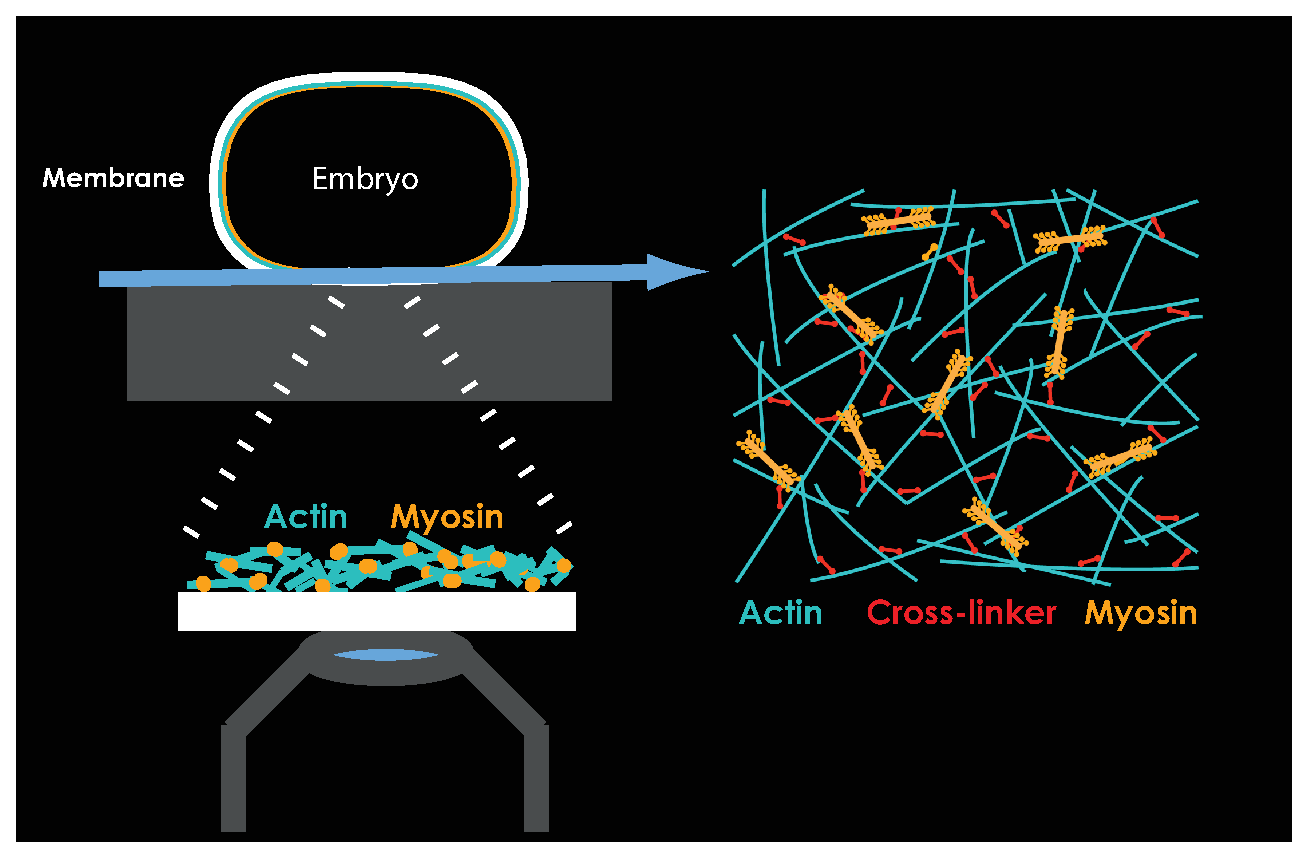
\includegraphics[width=0.85\textwidth]{Figure1-6}
\captionof{figure}[Schematic of experimental setup.]{\textbf{Schematic of experimental setup.} The cortex of 1 and 2-cell embryos was imaged using two-color near-TIRF microscopy.}
\end{figure}

\subsection{The significance of this thesis} 
The work presented in this thesis represents a significant contribution to our understanding of pulsed contractions.  We have identified what we believe constitutes a core set of proteins regulating pulsed contractions in \textit{C. elegans}.  Our experiments have demonstrated that pulsed contractions in \textit{C. elegans} are not primarily initiated by a contractile instability or clustering mechanism.  Instead, we have demonstrated that local activation and inactivation of RhoA regulates the initiation and termination pulsed contractions independent of myosin II-dependent contractility (see Chapter 2).  Further experiments demonstrate that tuning various effectors downstream of RhoA has a profound impact on actomyosin contractility as well as RhoA spatial dynamics (see Chapter 3).  The combination of these results suggest that RhoA spatial patterning is tightly coupled to cortical actomyosin contractility.  To explain these results, we describe a novel conceptual framework in which pulsed contractions are represented by an activator-inhibitor system in which the individual components undergo reactions, diffusion, and advections.  Coupling the inhibitor to the actomyosin cortex potentiates mechanical feedback onto RhoA  (see Chapter 4).  This novel framework has been synthesized from our own experiments, as well as important experimental and theoretical results from the Martin, Glotzer, Bement, and Grill groups.  We expect the results and ideas presented here to guide future investigations of pulsed contractions in particular, and other biological processes governed by mechanical regulation of RhoA in general (see Chapter 4).






\end{document}
					 				
			
		



